%Assumam, agora, condic~oes iniciais dadas por P(0) = Q(0) = 1 e considerem os casos seguintes
%Caso 1 a = b = k = 1, c = 0:5, d = 0:25, ` = 0:75
%Caso 2 a = b = k = 1, c = 0:75, d = 1, ` = 0:5
%Caso 3 a = b = k = 1, c = 1:5, d = 1, ` = 1
%Assumam, tambem, condic~oes iniciais dadas por P(0) = Q(0) = 2 e considerem o caso seguinte
%Caso 4 a = 0:1, b = 0:005, k = 0:001, c = 0:2, d =
%0:2
%120
%, ` = 0:02
%Estudem estes casos separadamente, acompanhando o seu estudo das simulac~oes que entendam
%apropriadas.




%Completar a sec¸c˜ao anterior com o estudo num´erico do modelo. An´alise quantitativa e qualitativa
%das solu¸c˜oes. Gr´aficos e leitura dos resultados.

\subsection{Simulações Numéricas}

\noindent
Posteriormente ao cálculo dos {\bf valores próprios} da matriz jacobiana em cada ponto de equilíbrio, usamos a tabela \ref{tab:template} para avaliarmos a sua {\bf estabilidade}.

\begin{table}[h!]

\vspace*{0.25cm}

\begin{center}
\begin{tabular}{| c | c | c | c | c |}
\hline \hline
  & \multicolumn{2}{| c |}{Sistema Linear} & \multicolumn{2}{| c |}{Sistema quase linear}\\ \hline \hline

{$r_1,r_2$}   &   {Tipo}   &  {Estabilidade} & {Tipo}   &  {Estabilidade}\\ \hline \hline
{$r_1>r_2>0$}  &  {N} & {Instável}  & {N} & {Instável}\\ \hline
{$r_1<r_2<0$}  &  {N} & {Assintoticamente estável}  & {N} & {Assintoticamente estável}\\ \hline
{$r_2<0<r_1$}  &  {SP} & {Instável}  & {SP} & {Instável}\\ \hline

{$r_1=r_2>0$}  &  {PN ou IN} & {Instável}  & {N ou SpP} & {Instável}\\ \hline
{$r_1=r_2<0$}  &  {PN ou IN} & {Assintoticamente estável}  & {N ou SpP} & {Assintoticamente estável}\\ \hline

{$r_1,r_2=\lambda+\pm\mu$}  &   &   &  & \\ \hline
{$\lambda >0$}  &  {spP} & {Instável}  & {SpP} & {Instável}\\ \hline
{$\lambda <0$}  &  {spP} & {Assintoticamente estável}  & {SpP} & {Assintoticamente estável}\\ \hline

{$r_1=i\mu, r_2=-i\mu$}  &  {C} & {Estável}  & {C ou SpP} & {Indeterminado}\\ \hline \hline


\multicolumn{5}{l}{\footnotesize{Nota: N, nó; IN, nó impróprio; PN, nó adequado; SP, ponto de sela; SpP, ponto espiral; C, centro.}} \\

%%%%%
\end{tabular}
\end{center}
\label{tab:template}
\caption{Propriedades de Estabilidade e Instabilidade de Sistemas Lineares e Quase Lineares \cite{boyce}.}
\end{table}

\pagebreak
%Para inserir uma figura, fazemos como na Figura \ref{fig:x}
\subsubsection{Caso 1}

As condições iniciais são: $P(0)=Q(0)=1$.\newline Os parâmetros são:  $a=b=k=1$, $c=0.5$, $d=0.25$, $\ell=0.75$.

%%%%%
\begin{figure}[htbp]
\centering
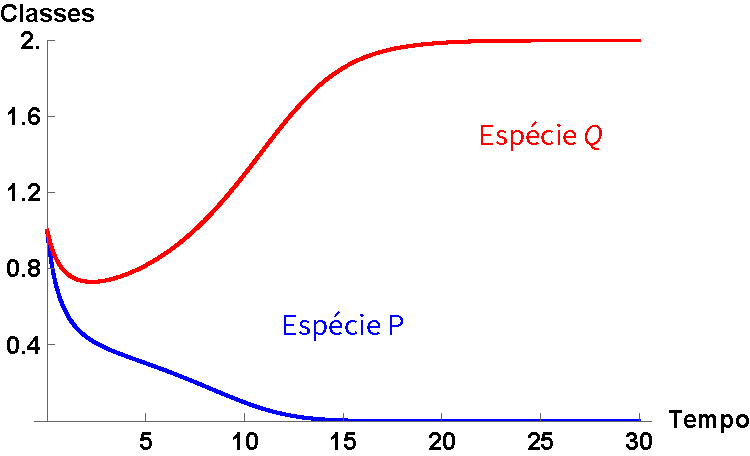
\includegraphics[keepaspectratio=true,scale=0.75]{caso1_a.pdf}
\caption{Solução numérica do sistema diferencial para o caso 1.}
\label{fig:x}
\end{figure}
\bigskip
\noindent
Comentario, Comentario,Comentario, Comentario,Comentario, Comentario,Comentario, Comentario,Comentario, Comentario,Comentario, Comentario,Comentario, Comentario,Comentario, Comentario,Comentario, Comentario,Comentario, Comentario,

%%%%%
\begin{figure}[htbp]
\centering
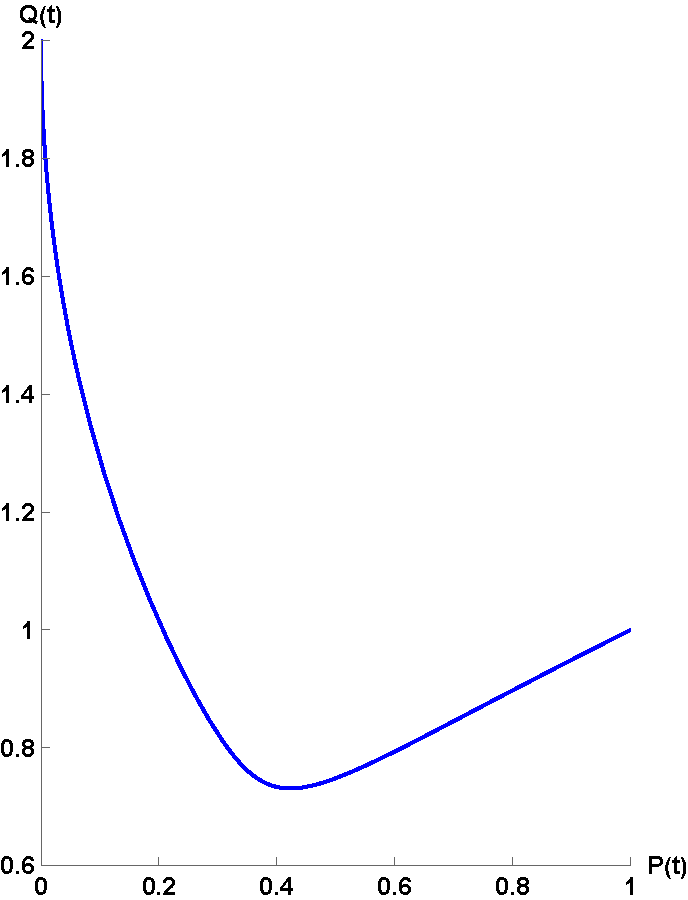
\includegraphics[keepaspectratio=true,scale=0.5]{caso1_b.pdf}
\caption{Esboço da relação entre P(t) e Q(t) para o caso 1.}
\label{fig:xx}
\end{figure}
\bigskip
\noindent
Comentario, Comentario,Comentario, Comentario,Comentario, Comentario,Comentario, Comentario,Comentario, Comentario,Comentario, Comentario,Comentario, Comentario,Comentario, Comentario,Comentario, Comentario,Comentario, Comentario,
\pagebreak


\begin{table}[h!]

\vspace*{0.25cm}

\begin{center}
\begin{tabular}{| c | c | c | c | c |}
\hline \hline
{Pontos de equilíbrio} & \multicolumn{2}{| c |}{Valores próprios} & {Tipo} & {Estabilidade}\\ \hline \hline

{$(0,0)$}   &   {$\lambda_1=0.5$} &   {$\lambda_2=1$}   &  {} & {Instável}\\ \hline

{$(0,2)$}   &   {$\lambda_1=-0.5$} &   {$\lambda_2=-1$}   &  {} & {Estável}\\ \hline

{$(1,0)$}   &   {$\lambda_1=-0.25$} &   {$\lambda_2=-1$}   &  {} & {Estável}\\ \hline

{$(0.5,0.5)$}   &   {$\lambda_1\cong-0.78$} &   {$\lambda_2\cong0.16$}   &  {Ponto de Sela} & {Instável}\\ \hline \hline

%%%%%
\end{tabular}
\end{center}
\label{tab:template}
\caption{Valores próprios e estabilidade por cada ponto de equilíbrio para o caso 1.}
\end{table}

\bigskip


\begin{figure}[htbp]
\centering
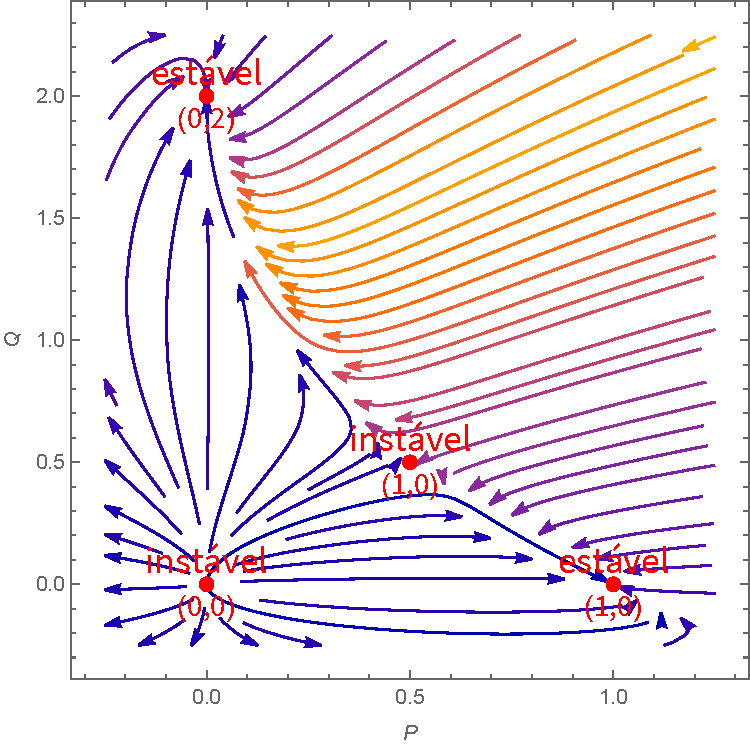
\includegraphics[keepaspectratio=true,scale=0.8]{caso1_c.pdf}
\caption{Campo de direções (com pontos de equilíbrio) para o caso 1.}
\label{fig:xxx}
\end{figure}
\bigskip
\noindent
Comentario, Comentario,Comentario, Comentario,Comentario, Comentario,Comentario, Comentario,Comentario, Comentario,Comentario, Comentario,Comentario, Comentario,Comentario, Comentario,Comentario, Comentario,Comentario, Comentario,
\pagebreak




















\subsubsection{Caso 2}


As condições iniciais são: $P(0)=Q(0)=1$.\newline Os parâmetros são:  $a=b=k=1$, $c=0.75$, $d=1$, $\ell=0.5$.
%%%%%
\begin{figure}[htbp]
\centering
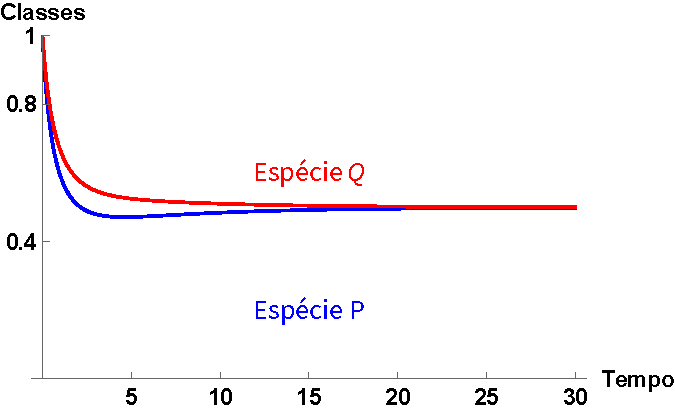
\includegraphics[keepaspectratio=true,scale=0.75]{caso2_a.pdf}
\caption{Solução numérica do sistema diferencial para o caso 2.}
\label{figy}
\end{figure}
\bigskip

\noindent
Comentario, Comentario,Comentario, Comentario,Comentario, Comentario,Comentario, Comentario,Comentario, Comentario,Comentario, Comentario,Comentario, Comentario,Comentario, Comentario,Comentario, Comentario,Comentario, Comentario,
%%%%%
\begin{figure}[htbp]
\centering
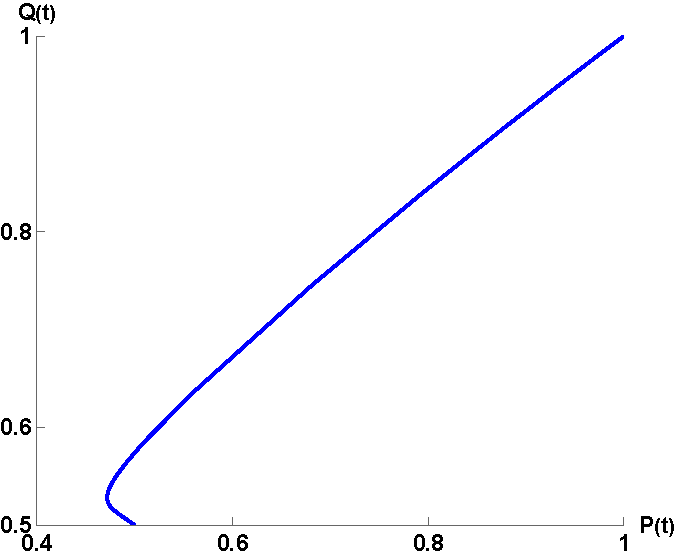
\includegraphics[keepaspectratio=true,scale=0.5]{caso2_b.pdf}
\caption{Esboço da relação entre P(t) e Q(t) para o caso 2.}
\label{fig:yy}
\end{figure}
\bigskip
\noindent
Comentario, Comentario,Comentario, Comentario,Comentario, Comentario,Comentario, Comentario,Comentario, Comentario,Comentario, Comentario,Comentario, Comentario,Comentario, Comentario,Comentario, Comentario,Comentario, Comentario,
\pagebreak
\begin{table}[h!]

\vspace*{0.25cm}

\begin{center}
\begin{tabular}{| c | c | c | c | c |}
\hline \hline
{Pontos de equilíbrio} & \multicolumn{2}{| c |}{Valores próprios} & {Tipo} & {Estabilidade}\\ \hline \hline

{$(0,0)$}   &   {$\lambda_1=0.75$} &   {$\lambda_2=1$}   &  {} & {Instável}\\ \hline

{$(0,0.75)$}   &   {$\lambda_1=-0.75$} &   {$\lambda_2=0.25$}   &  {Ponto de sela} & {Instável}\\ \hline

{$(1,0)$}   &   {$\lambda_1=-1$} &   {$\lambda_2=0.25$}   &  {Ponto de sela} & {Instável}\\ \hline

{$(0.5,0.5)$}   &   {$\lambda_1\cong-0.15$} &   {$\lambda_2\cong-0.86$}   &  {Ponto de Sela} & {Estável}\\ \hline \hline

%%%%%
\end{tabular}
\end{center}
\label{tab:template}
\caption{Valores próprios e estabilidade por cada ponto de equilíbrio para o caso 2.}
\end{table}

\bigskip
\begin{figure}[htbp]
\centering
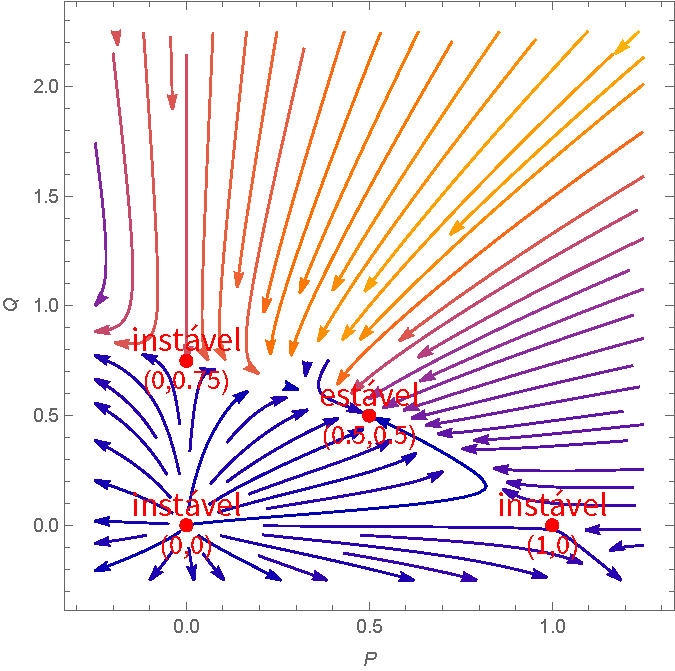
\includegraphics[keepaspectratio=true,scale=0.8]{caso2_c.pdf}
\caption{Campo de direções (com pontos de equilíbrio) para o caso 2.}
\label{fig:yyy}
\end{figure}
\bigskip
\noindent
Comentario, Comentario,Comentario, Comentario,Comentario, Comentario,Comentario, Comentario,Comentario, Comentario,Comentario, Comentario,Comentario, Comentario,Comentario, Comentario,Comentario, Comentario,Comentario, Comentario,




















\pagebreak
\subsubsection{Caso 3}


As condições iniciais são: $P(0)=Q(0)=1$.\newline Os parâmetros são:  $a=b=k=1$, $c=1.5$, $d=1$, $\ell=1$.
%%%%%
\begin{figure}[htbp]
\centering
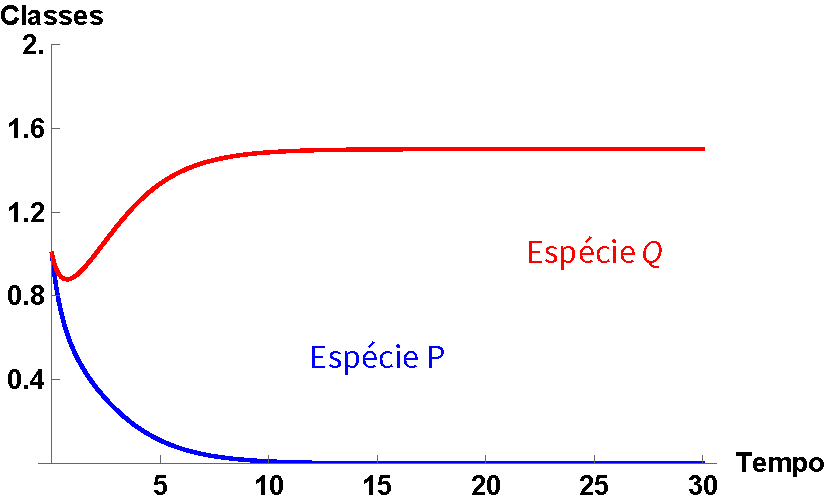
\includegraphics[keepaspectratio=true,scale=0.75]{caso3_a.pdf}
\caption{Solução numérica do sistema diferencial para o caso 3.}
\label{fig:z}
\end{figure}
\bigskip
\noindent
Comentario, Comentario,Comentario, Comentario,Comentario, Comentario,Comentario, Comentario,Comentario, Comentario,Comentario, Comentario,Comentario, Comentario,Comentario, Comentario,Comentario, Comentario,Comentario, Comentario,
\begin{figure}[htbp]
\centering
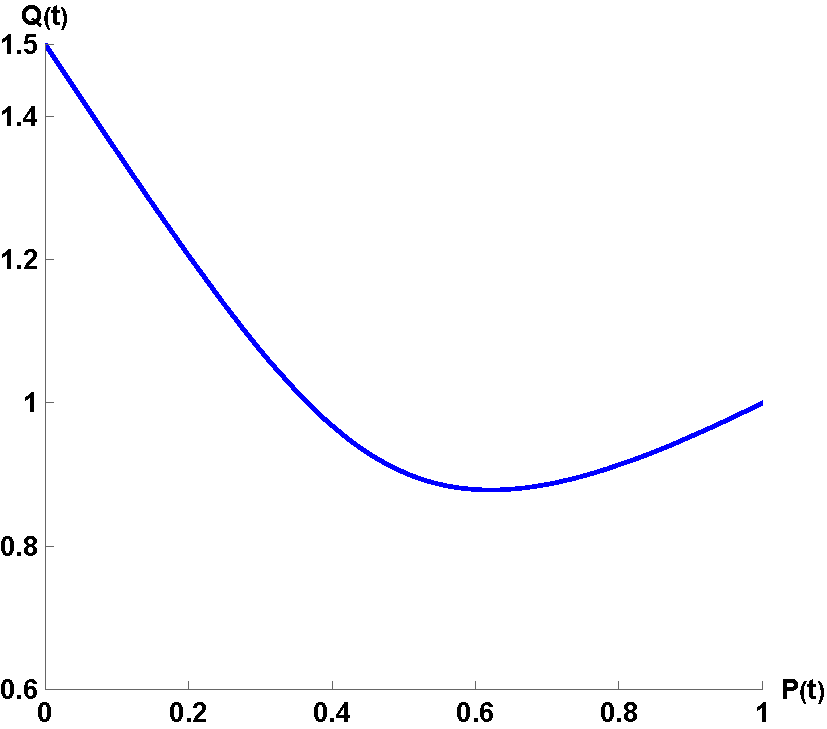
\includegraphics[keepaspectratio=true,scale=0.5]{caso3_b.pdf}
\caption{Esboço da relação entre P(t) e Q(t) para o caso 2.}
\label{fig:zz}
\end{figure}
\bigskip
\noindent
Comentario, Comentario,Comentario, Comentario,Comentario, Comentario,Comentario, Comentario,Comentario, Comentario,Comentario, Comentario,Comentario, Comentario,Comentario, Comentario,Comentario, Comentario,Comentario, Comentario,
\pagebreak
\begin{table}[h!]

\vspace*{0.25cm}

\begin{center}
\begin{tabular}{| c | c | c | c | c |}
\hline \hline
{Pontos de equilíbrio} & \multicolumn{2}{| c |}{Valores próprios} & {Tipo} & {Estabilidade}\\ \hline \hline

{$(0,0)$}   &   {$\lambda_1=1$} &   {$\lambda_2=1.5$}   &  {} & {Instável}\\ \hline

{$(0,1.5)$}   &   {$\lambda_1=-1.5$} &   {$\lambda_2=-0.5$}   &  {} & {Estável}\\ \hline

{$(1,0)$}   &   {$\lambda_1=-1.5$} &   {$\lambda_2=0.5$}   &  {Ponto de Sela} & {Instável}\\ \hline

{}   &   {} &   {}   &  {} & {}\\ \hline \hline

%%%%%
\end{tabular}
\end{center}
\label{tab:template}
\caption{Valores próprios e estabilidade por cada ponto de equilíbrio para o caso 3.}
\end{table}

\bigskip
%%%%%
\begin{figure}[htbp]
\centering
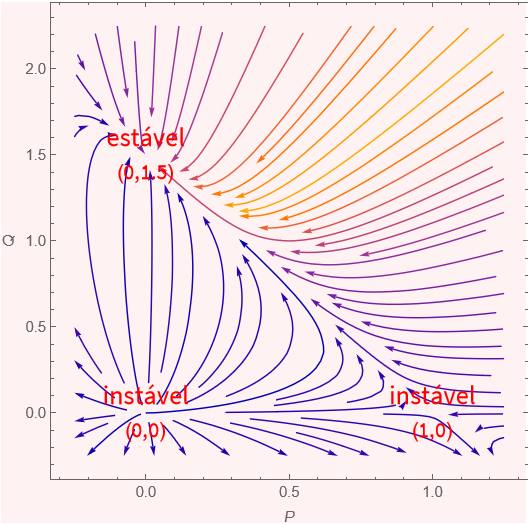
\includegraphics[keepaspectratio=true,scale=0.8]{caso3_c.jpg}
\caption{Campo de direções (com pontos de equilíbrio) para o caso 3.}
\label{fig:zzz}
\end{figure}
\bigskip
\noindent
Comentario, Comentario,Comentario, Comentario,Comentario, Comentario,Comentario, Comentario,Comentario, Comentario,Comentario, Comentario,Comentario, Comentario,Comentario, Comentario,Comentario, Comentario,Comentario, Comentario,

















\pagebreak
\subsubsection{Caso 4}


As condições iniciais são: $P(0)=Q(0)=2$.\newline Os parâmetros são:  $a=0.1$, $b=0.005$, $k=0.001$, $c=0.2$, $d=\frac{0.2}{120}$, $\ell=0.02$.
%%%%%
\begin{figure}[htbp]
\centering
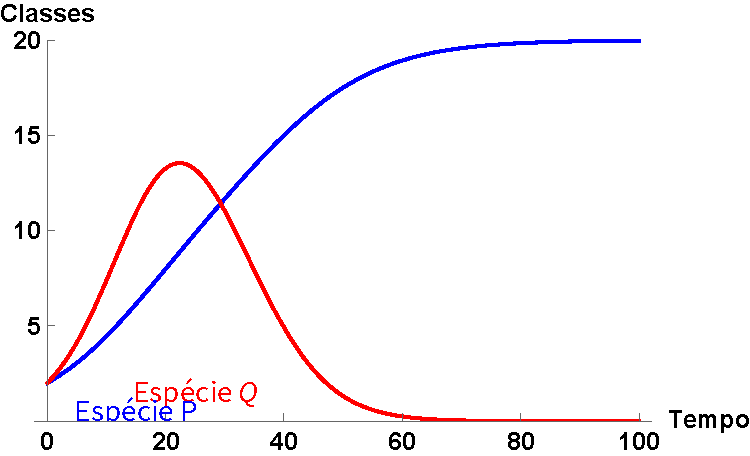
\includegraphics[keepaspectratio=true,scale=0.75]{caso4_a.pdf}
\caption{Solução numérica do sistema diferencial para o caso 4.}
\label{fig:w}
\end{figure}
\bigskip
\noindent
Comentario, Comentario,Comentario, Comentario,Comentario, Comentario,Comentario, Comentario,Comentario, Comentario,Comentario, Comentario,Comentario, Comentario,Comentario, Comentario,Comentario, Comentario,Comentario, Comentario,
%%%%%
\begin{figure}[htbp]
\centering
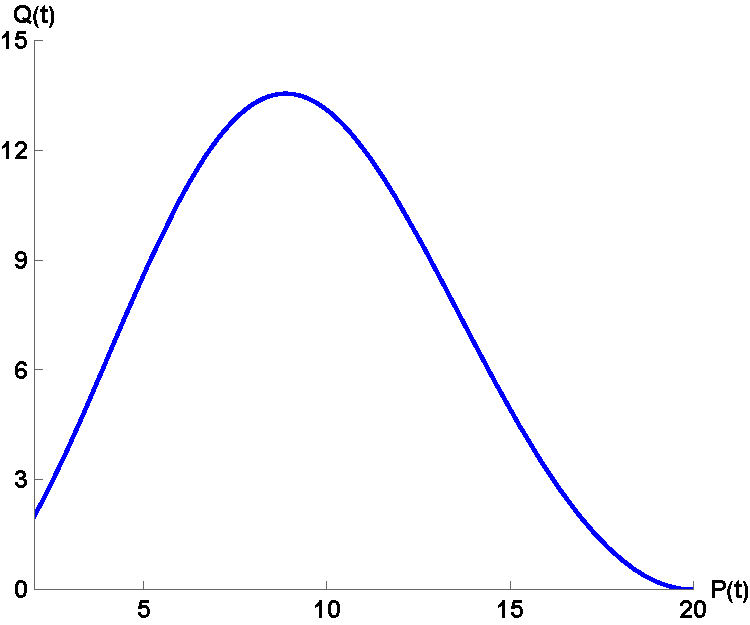
\includegraphics[keepaspectratio=true,scale=0.5]{caso4_b.pdf}
\caption{Esboço da relação entre P(t) e Q(t) para o caso 4.}
\label{fig:ww}
\end{figure}
\bigskip
\noindent
Comentario, Comentario,Comentario, Comentario,Comentario, Comentario,Comentario, Comentario,Comentario, Comentario,Comentario, Comentario,Comentario, Comentario,Comentario, Comentario,Comentario, Comentario,Comentario, Comentario,
\pagebreak
\begin{table}[h!]

\vspace*{0.25cm}

\begin{center}
\begin{tabular}{| c | c | c | c | c |}
\hline \hline
{Pontos de equilíbrio} & \multicolumn{2}{| c |}{Valores próprios} & {Tipo} & {Estabilidade}\\ \hline \hline

{$(0,0)$}   &   {$\lambda_1=0.1$} &   {$\lambda_2=0.2$}   &  {} & {Instável}\\ \hline

{$(0,120)$}   &   {$\lambda_1=-0.2$} &   {$\lambda_2=-0.02$}   &  {} & {Estável}\\ \hline

{$(20,0)$}   &   {$\lambda_1=-0.1$} &   {$\lambda_2=-0.2$}   &  {} & {Estável}\\ \hline

{$(2.86,85.7)$}   &   {$\lambda_1\cong-0.02$} &   {$\lambda_2\cong-0.17$}   &  {Ponto de Sela} & {Instável}\\ \hline \hline

%%%%%
\end{tabular}
\end{center}
\label{tab:template}
\caption{Valores próprios e estabilidade por cada ponto de equilíbrio para o caso 4.}
\end{table}

%%%%%
\begin{figure}[htbp]
\centering
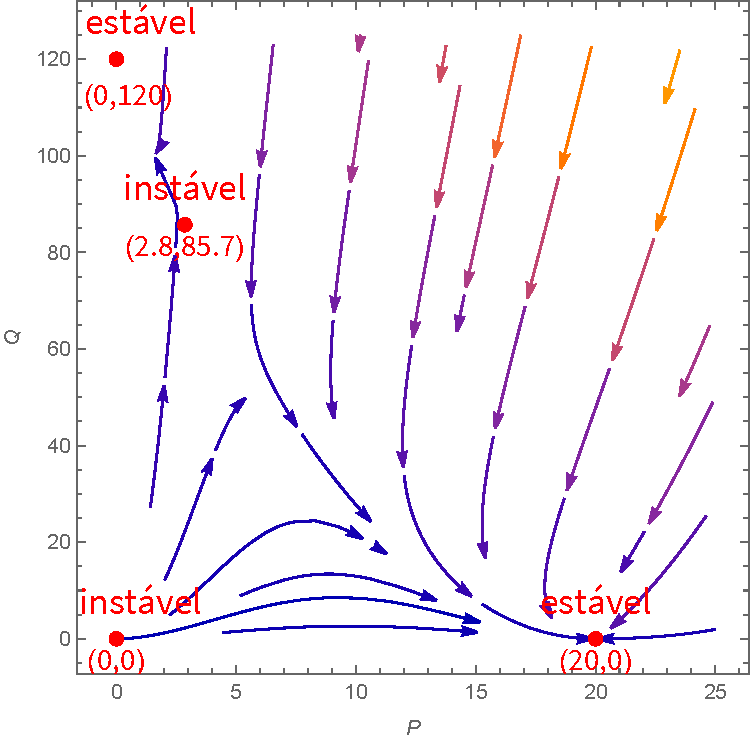
\includegraphics[keepaspectratio=true,scale=0.8]{caso4_c.pdf}
\caption{Campo de direções (com pontos de equilíbrio) para o caso 4.}
\label{fig:www}
\end{figure}
\bigskip
\noindent
Comentario, Comentario,Comentario, Comentario,Comentario, Comentario,Comentario, Comentario,Comentario, Comentario,Comentario, Comentario,Comentario, Comentario,Comentario, Comentario,Comentario, Comentario,Comentario, Comentario,

